%%%%%%%%%%%%%%%%%%%%%%%%%%%%%%%%%%%%%%
%%%%%%%%%%%%%%%%%%%%%%%%%%%%%%%%%%%%%%
% Do not edit the TeX file your work
% will be overwritten.  Edit the RnW
% file instead.
%%%%%%%%%%%%%%%%%%%%%%%%%%%%%%%%%%%%%%
%%%%%%%%%%%%%%%%%%%%%%%%%%%%%%%%%%%%%%



In this section, we apply our methods to Fisher's iris data set, using the
Gaussian mixture model (GMM) model from \exref{iris_bnp_process} and VB
approximation given in \eqref{vb_mf} and \exref{iris_var_distr}.  Here, the data
dimension $d = 4$, we set the truncation parameter $\kmax = 15$.  For our
quantities of interest, we investigate both the estimated number of in-sample
clusters as described in \exref{vb_insample_nclusters_simple} and the
\textit{posterior predictive} number of clusters. Let $\nclusters(\z)$ be the
number of clusters as defined as in \exref{insample_nclusters_simple}.  The
posterior predictive number of clusters, $\expect{\p(\pi \vert
\x)}{\expect{\p(\z \vert \pi)}{\nclusters(\z)}}$, is the posterior expectation
of the number of distinct clusters that we would expect to see in a new dataset
the same size as our original dataset.  Analogously to
\exref{insample_nclusters_simple}, we define a variational approximation to
posterior predictive number of clusters as
%
\begin{align*}
\gclusterspredabbr(\eta) :=
    \expect{\q(\nu\vert\eta)}{\expect{\p(\z\vert\nu)}{\nclusters(\z)}}
  = \sum_{k=1}^\kmax\left(1 -
  \expect{\q(\nu \vert \eta)}{(1 - \pi_\k)^\N} \right).
\end{align*}
%
In the iris example, the predictive quantity can interpreted as the expected
number of species one might see if a fresh sample of iris flowers were
collected.

\subsubsection*{Parametric sensitivity}

We first explore sensitivity of the in-sample and posterior predictive number of
clusters to the concentration parameter, $\alpha$, using the results in
\secref{diffable_concentration}.  To choose a plausible range of $\alpha$,
recall that, under the GEM$(\alpha)$ prior, the {\em a priori} expected
number of distinct clusters in a dataset of size $N$ is given
\citep{jordan:2015:gentleintrodp} by
%
\begin{align}\eqlabel{prior_num_clusters}
\expect{\p(\z \vert \pi)\p(\pi \vert \alpha)}{\nclusters(\z)} =
\sum_{\n = 1}^\N \frac{\alpha}{\alpha + \n - 1}.
\end{align}
%
Using this formula, we take $\alpha\in[0.1, 4.0]$, corresponding to an an {\em a
priori} range of approximately $1.5$ to $15$ clusters.  Over this range, the
shape of the stick-breaking density varies considerably, as shown in
\figref{beta_priors}.  We take $\alpha_0 = 2$, near the middle of the range, and
use the prior $\p(\nuk \vert \alpha_0)$ as the base prior at which we compute
the derivatives for all the results below.  \Figref{iris_fit} shows the
posterior clustering for $\alpha_0$.  For our base prior, the posterior thus
recovers the known ground truth that there are in truth three distinct species.


\begin{knitrout}
\definecolor{shadecolor}{rgb}{0.969, 0.969, 0.969}\color{fgcolor}\begin{figure}[!h]

{\centering 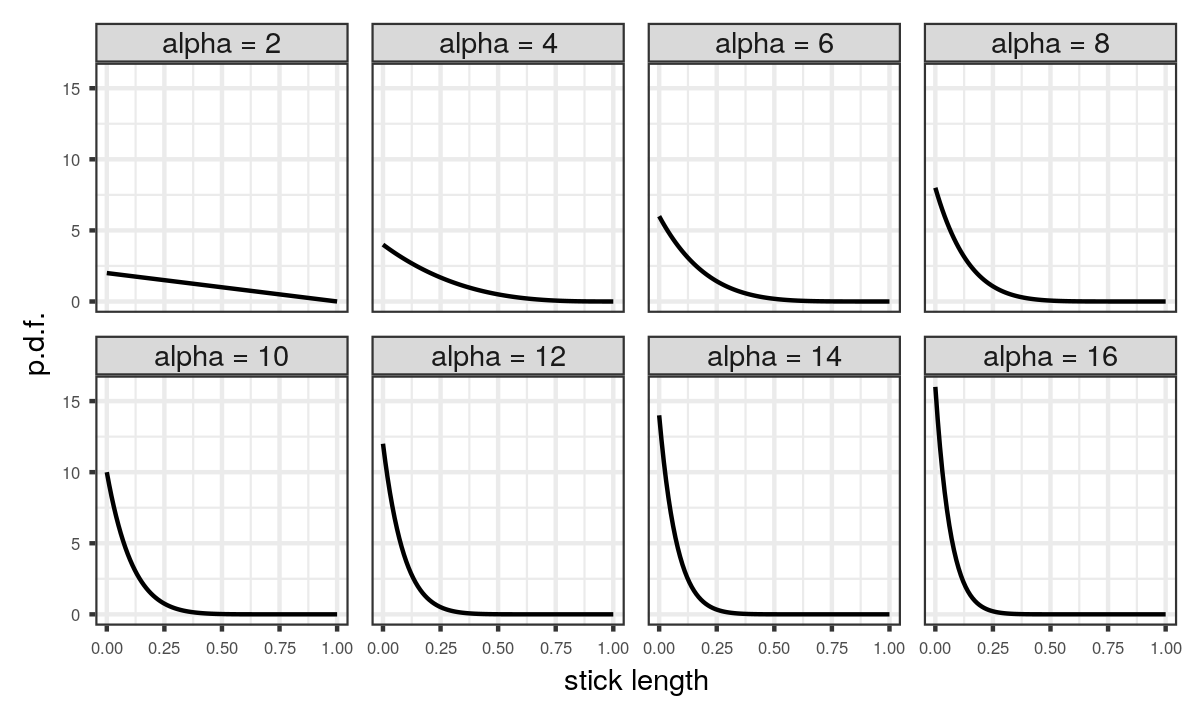
\includegraphics[width=0.980\linewidth,height=0.392\linewidth]{figure/beta_priors-1} 

}

\caption[Probability density functions of $\text{Beta}(1, \alpha)$ distributions, under various $\alpha$ considered for the iris data set]{Probability density functions of $\text{Beta}(1, \alpha)$ distributions, under various $\alpha$ considered for the iris data set.}\label{fig:beta_priors}
\end{figure}


\end{knitrout}



\begin{knitrout}
\definecolor{shadecolor}{rgb}{0.969, 0.969, 0.969}\color{fgcolor}\begin{figure}[!h]

{\centering 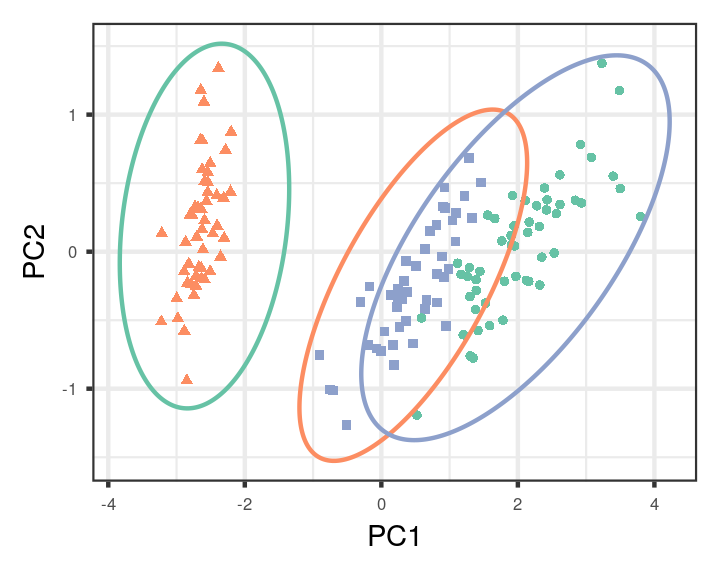
\includegraphics[width=0.588\linewidth,height=0.470\linewidth]{figure/iris_fit-1} 

}

\caption[The iris data in principal component space and
                      GMM fit at $\alpha = 2$]{The iris data in principal component space and
                      GMM fit at $\alpha = 2$. Colors denote inferred memberships and
                      ellipses represent estimated covariances. }\label{fig:iris_fit}
\end{figure}


\end{knitrout}



\begin{knitrout}
\definecolor{shadecolor}{rgb}{0.969, 0.969, 0.969}\color{fgcolor}\begin{figure}[!h]

{\centering 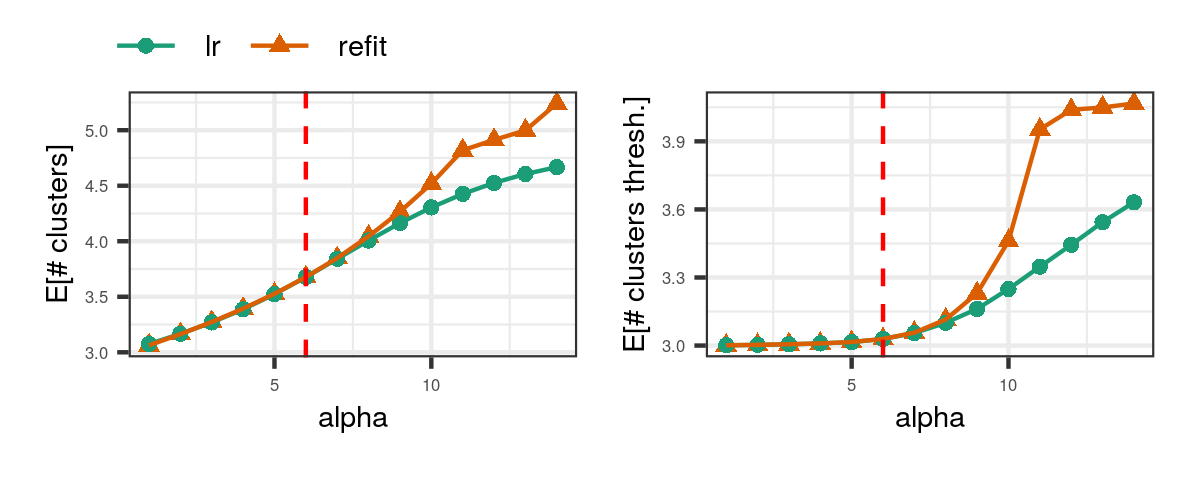
\includegraphics[width=0.784\linewidth,height=0.439\linewidth]{figure/iris_alpha_sens-1} 

}

\caption[The expected number of clusters as $\alpha$ varies in thethe GMM fit of the iris data]{The expected number of clusters as $\alpha$ varies in thethe GMM fit of the iris data. On the left is in-sample quantity $\gclustersabbr$. On the right is the the predictive quantity $\gclusterspredabbr$. We formed the linear approximation at $\alpha=2$.}\label{fig:iris_alpha_sens}
\end{figure}


\end{knitrout}

\Figref{iris_alpha_sens} shows both the posterior in-sample and predictive
number of distinct clusters as $\alpha$ varies.  Over this range of $\alpha$,
the in-sample number of clusters is quite robust, but the posterior predictive
number of clusters is non-robust, ranging roughly from 3.0 to 5.6 expected
species.  Our approximation captures this qualititative behavior. As expected,
the approximation is least accurate furthest from the $\alpha_0$ at which it is
evalutated.

Forming the linear approximation at $\alpha_0$ required 0.02 seconds, and, after forming the linear approximation,
computing $\etalinglobal(\alpha)$ for the sequence of $\alpha$'s considered in
\figref{iris_alpha_sens} took another 0.01 seconds. In contrast, to refit $\etaopt(\alpha)$ for the
set of $\alpha$s took a total of  9 seconds, with a median refit time of
0.5 seconds.  In this case, the
approximation produced the same qualitative conclusions an order of magnitude
faster than refitting.


\subsubsection*{Functional perturbations and the influence function}

\todo{Bryan: Why aren't we doing this with the predicted number of
clusters, which is actually sensitive?}

\todo{The reasoning here was: in-sample was insensitive to alpha. 
maybe sensitive to other functional perturbations?
Looks like its not, e.g. worst-case. 
TODO make this logic clear from the get-go}

In this section, we demonstrated the ability of the influence function to
predict the effect of nonparametric changes to the prior. As in the previous
section, we take $\pbase(\nuk) = \betadist(\nuk \vert 1, \alpha_0)$ for each
$\k$.  In order to facilitate visualization, we perform our computations in
logit-stick space.  In terms of \defref{prior_t}, we take $\mu$ to be the
Lebesgue measure on $\mathbb{R}^{\kmax - 1}$, and $\theta = (\lnu_1, \ldots,
\lnu_{\kmax - 1})$, suitably transforming the prior density.  Our quantity of
interest will be $\gclustersabbr$, the expected number of in-sample clusters.

\todo{A note for everywhere: it's not an inner product.  My bad for calling
it that at some point, but we need to get away from that.  It's just an
integral.  The reason is that the influence function may not be a
member of $L_\infty$; technically, it's a member of the dual space
($L_1$).}

\todo{Somewhere need to explain how the influence function is 1d despite
there being $\kmax - 1$ sticks}

The leftmost column of \figref{iris_fsens} shows in purple the influence
function, $\infl(\nu)$, as given by \corref{etafun_deriv_form}.  We consider
perturbations $\phi$ which are Gaussian bumps, with each perturbation centered
at a different location on the real line.  Each row of \figref{iris_fsens}
corresponds to a different $\phi$, which are shown in gray in the left-hand
column of \figref{iris_fsens}. The middle column of \figref{iris_fsens} shows
the stick-breaking prior $\p(\nuk \vert \phi)$ induced by the corresponding
$\phi$, and the rightmost column of \figref{iris_fsens} shows the changes
produced by the corresponding perturbation, as measured by re-fitting and  as
predicted by our approximation.

According to \corref{etafun_deriv_form}, the sign and magnitude of the effect of
a perturbation should be determined by its integral against the influence
function.  Thus, when $\phi$ lines up with a negative part of $\infl$, as in the
first row, we expect the change to be negative.  Similarly, we expect the
perturbation of the middle row to produce a positive change, and the bottom row,
in which $\phi$ overlaps with both negative and positive parts of the influence
function, to produce a relatively small change.  The third column of
\corref{etafun_deriv_form} confirms that this intuition holds.

\todo{This figure is actually pretty strange.  Why is it cut off?  Why is the
last row actually a pretty large negative change?}



\begin{knitrout}
\definecolor{shadecolor}{rgb}{0.969, 0.969, 0.969}\color{fgcolor}\begin{figure}[!h]

{\centering 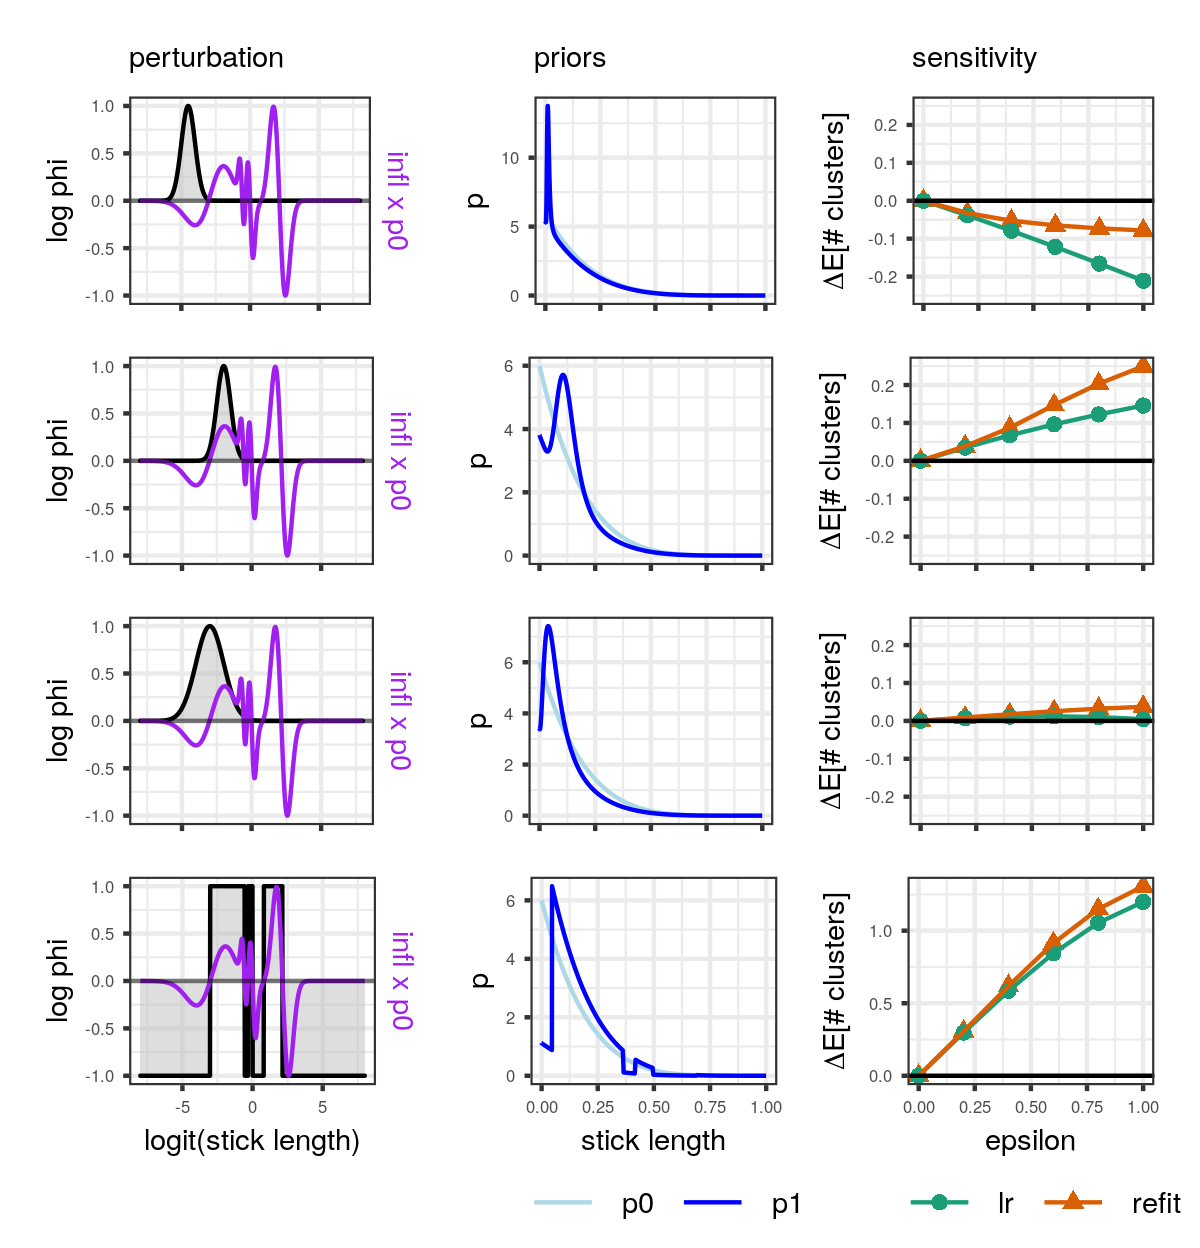
\includegraphics[width=0.980\linewidth,height=0.862\linewidth]{figure/iris_fsens-1} 

}

\caption{Sensitivity of
        the expected number of in-sample clusters
        in the iris data set
        to three multiplicative perturbations with
        unit $L_{\infty}$-norm.
        (Left) the multiplicative perturbation $\phi$ in grey.
        The influence function $\Psi$ in purple,
        scaled to also have unit $L_{\infty}$-norm.
        (Middle) the original prior density $\p_0$ and
        the perturbed prior density $\p_t = \p_0\times \exp(t \phi)$
        at $t = 1$.
        (Right) the effect of the perturbation
        on the change in expected number of in-sample clusters
        as $t\rightarrow1$.}\label{fig:iris_fsens}
\end{figure}


\end{knitrout}


\begin{knitrout}
\definecolor{shadecolor}{rgb}{0.969, 0.969, 0.969}\color{fgcolor}\begin{figure}[!h]

{\centering 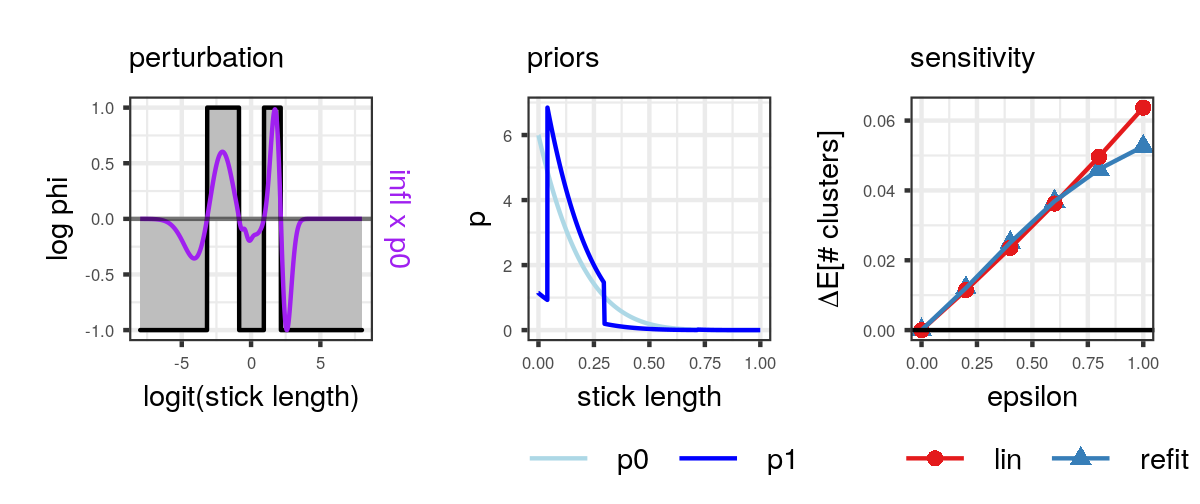
\includegraphics[width=0.980\linewidth,height=0.412\linewidth]{figure/iris_worstcase-1} 

}

\caption[Sensitivity of
        the expected number of in-sample clusters in the iris data set
        to the worst-case multiplicative perturbation with
        unit $L_{\infty}$-norm]{Sensitivity of
        the expected number of in-sample clusters in the iris data set
        to the worst-case multiplicative perturbation with
        unit $L_{\infty}$-norm.}\label{fig:iris_worstcase}
\end{figure}


\end{knitrout}



Finally, we consider the worst-case multiplicative perturbation with unit
$L_\infty$ norm. Recall that the worst-case perturbation with unit $L_\infty$
norm is a step-function taking on values $\pm1$ corresponding to the sign of the
influence function (\figref{iris_worstcase} left). The middle column of
\figref{iris_worstcase} shows the prior density perturbed by the worst-case
perturbation; the right column shows the effect on $\gclustersabbr$. This
worst-case perturbation has a much larger effect on $\gclustersabbr$ compared to
the other unit $L_\infty$ norm perturbations in \figref{iris_fsens}. However,
even with the worst-case perturbation, the change in $\gclustersabbr$ is still
small. We conclude that on the iris data set, $\gclustersabbr$ appears to be a
quantity insensitive to the prior under a Gaussian mixture model.






Computing the linearized variational parameters $\etalinglobal(\t)$ at $\t = 1$
(including the necessary Hessian solve)
for a given functional perturbation
required 0.03 seconds.
A refit at $\t = 1$ requires about one second.
While a second for a refit is not exceedingly large, the
order-of-magnitude difference in timing between the linear approximation and refit
will continue to hold for larger data analysis problems below.
In general, the speed of the linear approximation allows us to quickly
explore many different potential functional perturbations when
refitting for each perturbation becomes prohibitive.
In the data applications below,
the influence function will guide our choice of functional perturbation and
uncover potentially influential perturbations.

% \begin{table}[tb]
% \centering
% \caption{Compute time of results on the iris data set. }
% \begin{tabular}{|r|r|}
%     \hline
%     & time (seconds) \\
%     \hline
%     Initial fit & sprintf('%1.2g', init_fit_time) \\
%     \hline
%     Hessian solve for $\alpha$ sensitivity &
%         sprintf('%1.2g', alpha_hess_time)\\
%     Linear approx. $\eta^{lin}(\alpha)$ for $\alpha = 1, \ldots , 16$ &
%         sprintf('%1.2g', total_alpha_lr_time)\\
%     Refits $\eta(\alpha)$ for $\alpha = 1, \ldots , 16$ &
%         sprintf('%1.2g', total_alpha_refit_time)\\
%     \hline
%     The influence function & sprintf('%1.2g', infl_time)\\
%     Hessian solve for worst-case $\phi$ &
%         sprintf('%1.2g', wc_hessian_time)\\
%     Linear approx. $\eta^{lin}(\t)|_{\t = 1}$
%     for worst-case $\phi$ &
%         sprintf('%1.2g', wc_lr_time)\\
%     Refit $\eta(\t)|_{\t = 1}$ for worst-case $\phi$ &
%         sprintf('%1.2g', wc_refit_time)\\
%     \hline
% \end{tabular}
% \end{table}
